% Directed weighted graph for Bellman-Ford example.
\documentclass[tikz,border=2pt]{standalone}
\usepackage{tikz}
\usetikzlibrary{positioning,arrows.meta}

\begin{document}
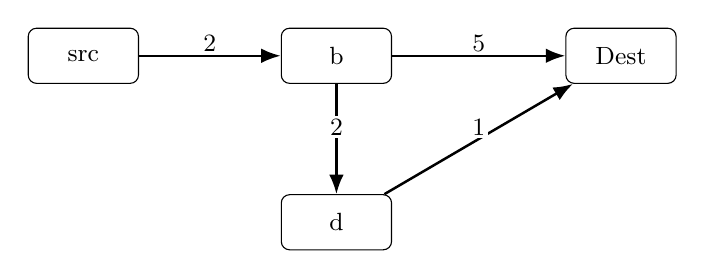
\begin{tikzpicture}[
  >=Latex,
  node/.style={draw, rounded corners=3pt, minimum width=14mm, minimum height=7mm, align=center, font=\small},
  edge/.style={->, line width=0.9pt},
  w/.style={font=\small, fill=white, inner sep=1pt}
]
  \node[node] (src) {src};
  \node[node, right=18mm of src] (b) {b};
  \node[node, right=22mm of b] (dest) {Dest};
  \node[node, below=14mm of b] (d) {d};

  \draw[edge] (src) -- node[w, midway, above] {2} (b);
  \draw[edge] (b) -- node[w, midway, above] {5} (dest);
  \draw[edge] (b) -- node[w, midway, above] {2} (d);
  \draw[edge] (d) -- node[w, midway, above] {1} (dest);
\end{tikzpicture}
\end{document}

